%! TeX root = master.tex
% !TEX program = lualatex

\lecture{3}{2026-09-23}{Concentration of Measure and Explore-then-Commit}{}

\section{Concentration of Measure}

\subsection{Motivation: sums of i.i.d.\ random variables}

To analyze bandit algorithms, we have to deal with sums of random rewards (hence of random regrets). The building block is the following setting.

Let $X_1, X_2, \dots, X_n$ be i.i.d.\ random variables whose mean and variance exist:
\[
\mu = \mathbb{E}[X], \qquad \sigma^2 = \mathbb{V}[X] = \mathbb{E}\big[(X - \mathbb{E}[X])^2\big].
\]
A natural \emph{estimator} of $\mu$ is the empirical mean
\[
\hat{\mu} = \frac{1}{n}\sum_{i=1}^n X_i =: \frac{S_n}{n}.
\]
It satisfies:
\begin{itemize}
    \item $\mathbb{E}[\hat{\mu}] = \mu$: $\hat{\mu}$ is an \emph{unbiased} estimator;
    \item $\mathbb{V}[\hat{\mu}] = \mathbb{E}\big[(\hat{\mu} - \mu)^2\big] = \dfrac{\sigma^2}{n}$: the variance of the estimator decreases with $n$.
\end{itemize}

The question of this chapter is: \emph{how close to $\mu$ is $\hat{\mu}$, with what probability, and for a given finite $n$?} We go through increasingly precise answers: law of large numbers, central limit theorem, Markov/Chebyshev inequalities, and finally exponential (Chernoff-type) bounds valid for finite $n$.

\subsection{Large $n$ limits}

\subsubsection*{Law of large numbers (LLN)}

\begin{theorem}[Law of large numbers]
Let $X_1, \dots, X_n$ be i.i.d.\ with mean $\mu$.
\begin{itemize}
    \item \textbf{Weak law}: for every $\epsilon > 0$, $\displaystyle \lim_{n \to \infty} \mathbb{P}\big(|S_n - n\mu| \geq n\epsilon\big) = 0$.
    \item \textbf{Strong law}: $\displaystyle \mathbb{P}\left(\lim_{n \to \infty} \frac{S_n}{n} = \mu\right) = 1$.
\end{itemize}
\end{theorem}

\begin{remark}[Two notions of convergence]
  The weak law is a statement of \emph{convergence in probability}, the strong law a statement of \emph{almost sure convergence}. The latter is strictly stronger. \\ \textit{Example} of a (non i.i.d.) sequence that converges to $0$ in probability but not almost surely: let the $Y_n$ be independent with $Y_n = 1$ with probability $1/n$ and $Y_n = 0$ otherwise. Then $\mathbb{P}(Y_n = 1) = 1/n \to 0$, so $Y_n \to 0$ in probability; but since $\sum_n 1/n = \infty$, almost every trajectory $\omega$ contains infinitely many $1$'s, so $Y_n(\omega)$ does not converge to $0$.
\end{remark}

\begin{center}
  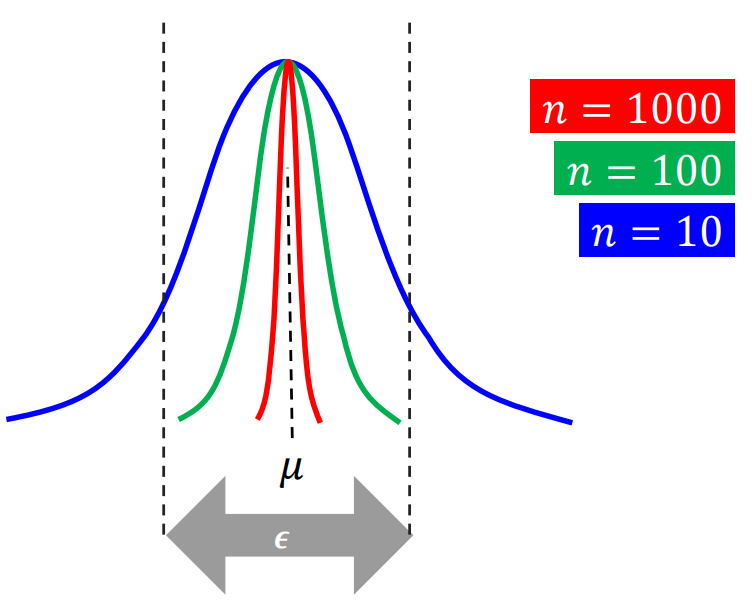
\includegraphics[width=0.4\linewidth]{images/img_20260930_163102.png}
\end{center}

Note that the LLN is an \emph{asymptotic} statement ($n \to \infty$): it says nothing about the probability of a deviation for a specific finite $n$.

\subsubsection*{Central limit theorem (CLT)}

The LLN says that $S_n/n$ concentrates around $\mu$. The CLT tells us at which \emph{scale}: rescale $\hat{\mu} - \mu$ by the inverse of its standard deviation ($1/\sqrt{n}$), i.e., look at $S_n - n\mu$ divided by $\sqrt{n}$:
\[
\frac{S_n - n\mu}{\sqrt{n}} \xrightarrow{n \to \infty} \mathcal{N}(0, \sigma^2).
\]
Equivalently, for large $n$, $\mathbb{P}\big(S_n - n\mu \geq n\epsilon\big) \to \mathbb{P}\big(\mathcal{N}(0,\sigma^2) \geq \epsilon\sqrt{n}\big)$.

This is the primary reason why the Gaussian law is so central (in addition to its stability under addition).

\begin{center}
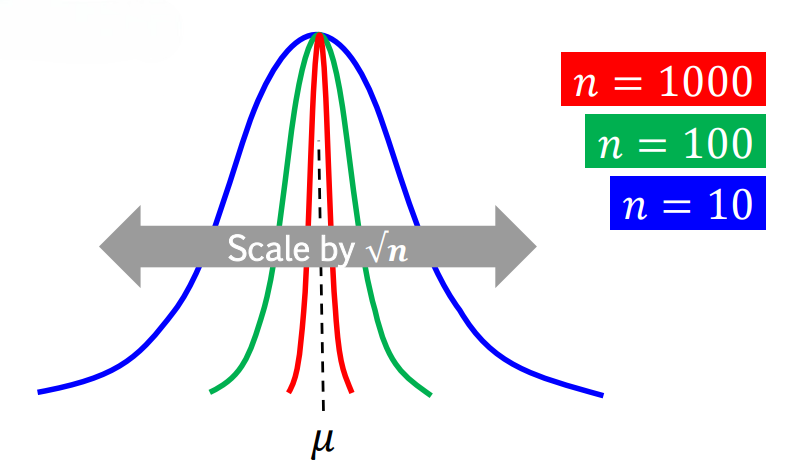
\includegraphics[width=0.4\linewidth]{images/img_20260930_163935.png}
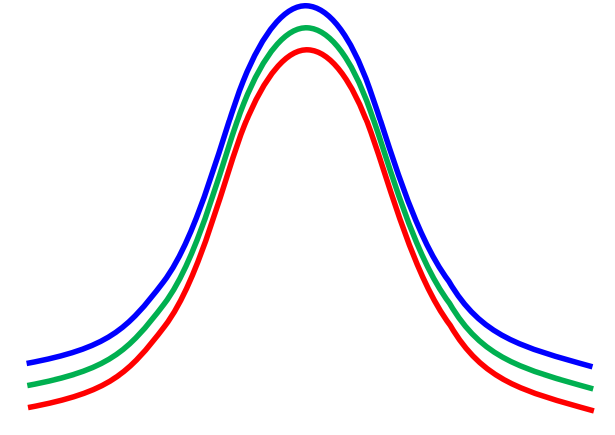
\includegraphics[width=0.3\linewidth]{images/img_20260930_163819.png}
\end{center}

\subsection{Markov and Chebyshev inequalities}

\begin{theorem}[Markov's inequality]
For any random variable $X$ and any $\epsilon > 0$,
\[
\mathbb{P}(|X| \geq \epsilon) \leq \frac{\mathbb{E}|X|}{\epsilon}.
\]
\end{theorem}

\begin{proof}
Set $Y = |X| \geq 0$ with density $f$. Then
\[
\mathbb{E}[Y] = \int_0^\infty y f(y)\, dy \geq \int_\epsilon^\infty y f(y)\, dy \geq \epsilon \int_\epsilon^\infty f(y)\, dy = \epsilon\, \mathbb{P}(Y \geq \epsilon).
\]
\end{proof}

\begin{theorem}[Chebyshev's inequality]
For any random variable $X$ with finite variance and any $\epsilon > 0$,
\[
\mathbb{P}\big(|X - \mathbb{E}X| \geq \epsilon\big) \leq \frac{\mathbb{V}[X]}{\epsilon^2}.
\]
\end{theorem}

\begin{proof}
Apply Markov's inequality to the non-negative random variable $(X - \mathbb{E}X)^2$ with threshold $\epsilon^2$.
\end{proof}

Applied to the empirical mean (whose variance is $\sigma^2/n$):
\[
\mathbb{P}\big(|\hat{\mu} - \mu| \geq \epsilon\big) \leq \frac{\sigma^2}{n\epsilon^2}.
\]

\begin{itemize}
    \item \textbf{Pro}: a nice, very general bound: only the mean and the variance are needed, and it holds for every finite $n$.
    \item \textbf{Con}: the bound is loose, it only decreases as $1/n$.
\end{itemize}
We need something much stronger for a meaningful analysis of bandit algorithms.

\subsection{Gaussian tail from the CLT}

By the CLT, $\dfrac{S_n - n\mu}{\sqrt{n\sigma^2}} \to \mathcal{N}(0,1)$. What if the normalized sum were \emph{exactly} Gaussian? Let $Z \sim \mathcal{N}(0,1)$; we want to bound
\[
\mathbb{P}(Z \geq z) = \int_z^\infty \frac{1}{\sqrt{2\pi}} \exp\left(-\frac{x^2}{2}\right) dx.
\]
This integral has no closed form, so we look for a bound. Since $x/z \geq 1$ on the domain of integration ($x \geq z > 0$),
\[
\int_z^\infty \frac{1}{\sqrt{2\pi}} e^{-x^2/2}\, dx \leq \frac{1}{\sqrt{2\pi}} \int_z^\infty \frac{x}{z}\, e^{-x^2/2}\, dx = \frac{1}{\sqrt{2\pi}\, z} \exp\left(-\frac{z^2}{2}\right).
\]

Now, using $\hat{\mu} - \mu = \dfrac{S_n - n\mu}{n}$ and taking $z = \epsilon\sqrt{n/\sigma^2}$, the CLT heuristic gives
\[
\mathbb{P}(\hat{\mu} - \mu \geq \epsilon) \;\longrightarrow\; \mathbb{P}\left(Z \geq \epsilon\sqrt{\tfrac{n}{\sigma^2}}\right) \leq \sqrt{\frac{\sigma^2}{2\pi n \epsilon^2}}\, \exp\left(-\frac{n\epsilon^2}{2\sigma^2}\right).
\]

\begin{itemize}
    \item \textbf{Pro}: much tighter than Chebyshev in general -- \emph{exponential} in $n$ versus $1/n$.
    \item \textbf{Con}: this is an \emph{asymptotic} result: the CLT does not allow us to bound the probability for a finite $n$.
\end{itemize}
We will need to pay for this limitation by making additional assumptions on the noise: \textbf{subgaussianity}.

\subsection{Subgaussian random variables}

\begin{definition}[Subgaussian random variable]
A random variable $X$ is \emph{$\sigma$-subgaussian} if its moment-generating function $M_X(\lambda) = \mathbb{E}[e^{\lambda X}]$ satisfies, for all $\lambda \in \mathbb{R}$,
\[
M_X(\lambda) = \mathbb{E}\big[e^{\lambda X}\big] \leq \exp\left(\frac{\lambda^2\sigma^2}{2}\right).
\]
Equivalently, in terms of the cumulant-generating function, \[
  \psi_X(\lambda) = \log M_X(\lambda) \leq \frac{1}{2}\lambda^2\sigma^2
\] for all $\lambda \in \mathbb{R}$.
\end{definition}

\begin{remark}
\begin{itemize}
    \item If $X$ is $\sigma$-subgaussian, then it is also $\sigma'$-subgaussian for any $\sigma' > \sigma$.
    \item Interpretation: the right-hand side $\exp(\lambda^2\sigma^2/2)$ is exactly the MGF of $\mathcal{N}(0,\sigma^2)$. A subgaussian variable has an MGF dominated by that of a Gaussian, i.e., its tail is at least as light as a Gaussian tail: ``nice'' noise with ``no big excesses''.
    \item Three cases can be distinguished: \emph{heavy-tailed} variables ($M_X(\lambda) = \infty$ for all $\lambda \neq 0$), \emph{light-tailed but not subgaussian} ($M_X(\lambda) < \infty$ on a neighborhood of $0$ but $M_X(\lambda) = \infty$ for large $|\lambda|$, or $M_X$ not dominated by the Gaussian one), and \emph{light-tailed and subgaussian} ($M_X(\lambda) \leq \exp(\lambda^2\sigma^2/2)$ for all $\lambda$).
\end{itemize}
\end{remark}

\begin{center}
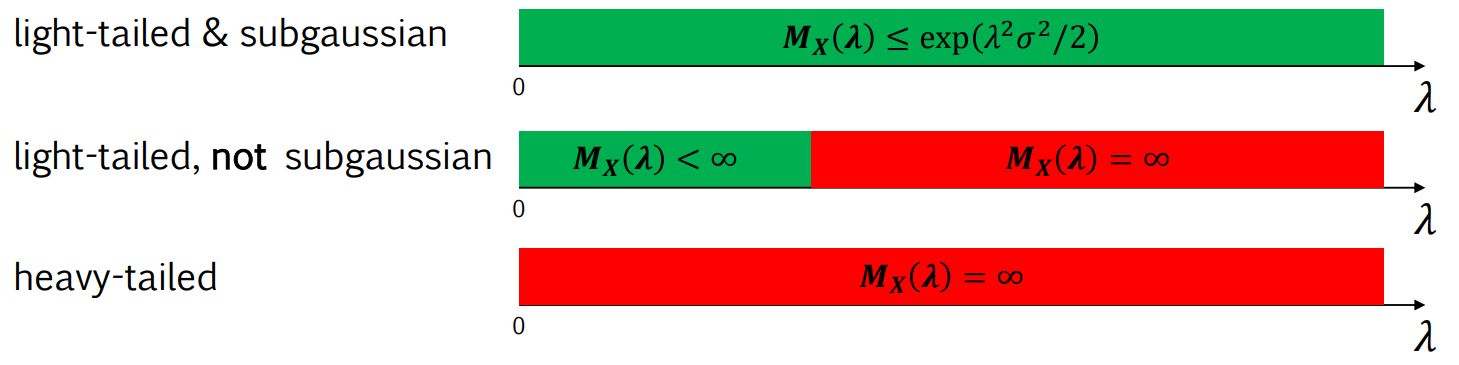
\includegraphics[width=0.8\linewidth]{images/img_20260930_170411.png}
\end{center}

\subsubsection*{Properties of subgaussian random variables}

\begin{lemma}
Assume $X$ is $\sigma$-subgaussian. Then:
\begin{enumerate}[label=(\alph*)]
  \item $\mathbb{E}[X] = 0$ and $\mathbb{V}[X] \le \sigma^2$;
  \item for any $\alpha \in \mathbb{R}$, $\alpha X$ is $|\alpha|\sigma$-subgaussian;
  \item if $X_1$ is $\sigma_1$-subgaussian, $X_2$ is $\sigma_2$-subgaussian and $X_1 \perp X_2$, then $X_1 + X_2$ is $\sqrt{\sigma_1^2 + \sigma_2^2}$-subgaussian.
\end{enumerate}
\end{lemma}

\begin{remark}[Abuse of notation]

We sometimes refer to subgaussian random variables that are \emph{not} zero-mean; by this we mean that $X - \mathbb{E}X$ is subgaussian.
\end{remark}

\begin{proof}[Proof of (a), sketch]
Compare the Taylor expansions of both sides of $\mathbb{E}[e^{\lambda X}] \leq \exp(\lambda^2\sigma^2/2)$ around $\lambda = 0$. On the left,
\[
e^{\lambda X} = 1 + \lambda X + \frac{\lambda^2 X^2}{2} + o(\lambda^2) \;\Longrightarrow\; \mathbb{E}\big[e^{\lambda X}\big] = 1 + \lambda\,\mathbb{E}X + \frac{\lambda^2\,\mathbb{E}X^2}{2} + o(\lambda^2),
\]
and, once we know $\mathbb{E}X = 0$ (the linear term in $\lambda$ must vanish, otherwise the inequality would fail for small $\lambda$ of the appropriate sign), $\mathbb{E}X^2 = \mathbb{V}X$, so the left side equals $1 + \frac{\lambda^2}{2}\mathbb{V}X + o(\lambda^2)$. On the right, $\exp(\lambda^2\sigma^2/2) = 1 + \frac{\sigma^2\lambda^2}{2} + o(\lambda^2)$. Hence
\[
\mathbb{V}X + \frac{o(\lambda^2)}{\lambda^2/2} \leq \sigma^2 + \frac{o(\lambda^2)}{\lambda^2/2},
\]
and taking $\lambda \to 0$ gives $\mathbb{V}X \leq \sigma^2$.

(b) follows since $\mathbb{E}[e^{\lambda\alpha X}] \leq \exp(\lambda^2\alpha^2\sigma^2/2)$; (c) follows from independence: $\mathbb{E}[e^{\lambda(X_1 + X_2)}] = \mathbb{E}[e^{\lambda X_1}]\,\mathbb{E}[e^{\lambda X_2}] \leq \exp\big(\lambda^2(\sigma_1^2 + \sigma_2^2)/2\big)$.
\end{proof}

\subsection{Tail of a subgaussian random variable}

\begin{theorem}[Tail bound]
If $X$ is $\sigma$-subgaussian, then for all $\epsilon > 0$,
\[
\mathbb{P}(X \geq \epsilon) \leq \exp\left(-\frac{\epsilon^2}{2\sigma^2}\right).
\]
\end{theorem}

\begin{proof}
Let $\lambda > 0$. By monotonicity of $\exp$, then Markov's inequality, then the definition of subgaussianity,
\begin{align*}
\mathbb{P}(X \geq \epsilon) &= \mathbb{P}\big(\exp(\lambda X) \geq \exp(\lambda\epsilon)\big) \\
&\leq \mathbb{E}\big[\exp(\lambda X)\big]\, \exp(-\lambda\epsilon) \\
&\leq \exp\left(\frac{\lambda^2\sigma^2}{2} - \lambda\epsilon\right).
\end{align*}
This holds for all $\lambda > 0$, so we may choose $\lambda$ freely: taking $\lambda = \epsilon/\sigma^2$ (the minimizer of the exponent) gives $\exp\!\big(-\epsilon^2/(2\sigma^2)\big)$.
\end{proof}

The same argument gives the corresponding inequality for the left tail, so that, combining both tails (union bound),
\[
\mathbb{P}(|X| \geq \epsilon) \leq 2\exp\left(-\frac{\epsilon^2}{2\sigma^2}\right).
\]

\subsubsection*{Confidence intervals}

Inverting this relationship gives \emph{confidence intervals} for $X$. Fix a small probability (error tolerance) $\delta \in (0,1)$. Solving $\exp(-\epsilon^2/(2\sigma^2)) = \delta$ for $\epsilon$:
\[
\mathbb{P}\left(X \geq \sqrt{2\sigma^2\ln(1/\delta)}\right) \leq \delta.
\]
For the two-sided version, we use the \textbf{union bound} $\mathbb{P}(A \cup B) \leq \mathbb{P}(A) + \mathbb{P}(B)$, which yields the factor $2$:
\[
\mathbb{P}\left(|X| \geq \sqrt{2\sigma^2\ln(2/\delta)}\right) \leq \delta.
\]
So, with probability at least $1 - \delta$, $X$ concentrates in the confidence interval
\[
\left[-\sqrt{2\sigma^2\ln\tfrac{2}{\delta}},\; +\sqrt{2\sigma^2\ln\tfrac{2}{\delta}}\right].
\]
We will apply such confidence intervals to characterize the estimators of per-arm reward in different bandit algorithms.

\subsection{Large deviation bound for finite $n$}

\begin{theorem}[Concentration of the empirical mean]
Assume that $X_i - \mu$, $i = 1,\dots,n$, are independent $\sigma$-subgaussian random variables. Then for any $\epsilon > 0$,
\[
\mathbb{P}(\hat{\mu} \geq \mu + \epsilon) \leq \exp\left(-\frac{n\epsilon^2}{2\sigma^2}\right).
\]
\end{theorem}

\begin{proof}
$\hat{\mu} - \mu = \frac{1}{n}\sum_{i=1}^n (X_i - \mu)$ is $\sigma/\sqrt{n}$-subgaussian (by properties (b) and (c): the sum is $\sqrt{n}\sigma$-subgaussian, and scaling by $1/n$ gives $\sigma/\sqrt{n}$). Apply the tail bound of the previous theorem with parameter $\sigma/\sqrt{n}$.
\end{proof}

Equivalently, $\mathbb{P}(S_n - n\mu \geq n\epsilon) \leq \exp\big(-n\epsilon^2/(2\sigma^2)\big)$. This is a bound similar to what the CLT suggests, but this time it is a true bound valid for every finite $n$ -- at the price of applying only to a (much smaller) class of variables. On a semi-log plot, the bound is a straight line in $n$ with slope $-\epsilon^2/(2\sigma^2)$.

\textbf{Confidence intervals for the mean.} Inverting as before:
\[
\mathbb{P}\left(\mu \geq \hat{\mu} + \sqrt{\frac{2\sigma^2\ln(1/\delta)}{n}}\right) \leq \delta, \qquad \mathbb{P}\left(\mu \leq \hat{\mu} - \sqrt{\frac{2\sigma^2\ln(1/\delta)}{n}}\right) \leq \delta,
\]
and, two-sided,
\[
\mathbb{P}\left(\mu \in \left[\hat{\mu} - \sqrt{\frac{2\sigma^2\ln(2/\delta)}{n}},\; \hat{\mu} + \sqrt{\frac{2\sigma^2\ln(2/\delta)}{n}}\right]\right) \geq 1 - \delta.
\]
The width of the interval shrinks as $1/\sqrt{n}$ and grows only as $\sqrt{\ln(1/\delta)}$ when we demand more confidence.

\subsection{Examples of subgaussian random variables}

\begin{itemize}
    \item \textbf{Gaussian is subgaussian}: $X \sim \mathcal{N}(0,\sigma^2)$ has $M_X(\lambda) = \exp(\lambda^2\sigma^2/2)$, hence is $\sigma$-subgaussian (with equality in the definition).
    \item \textbf{Bounded is subgaussian}: if $X \in [a,b]$ almost surely, then $X$ is $\frac{b-a}{2}$-subgaussian (Hoeffding's lemma). \\ In particular, if $|X| \leq a$ almost surely, then $X$ is $a$-subgaussian. For instance, a Bernoulli variable is $\frac{1}{2}$-subgaussian.
    \item \textbf{Exponential is \emph{not} subgaussian} (its tail is not light enough!): for $X \sim \mathrm{Exp}(1/\mu)$ (mean $\mu$),
    \[
    M_X(\lambda) = \int_0^\infty \mu^{-1} e^{-x/\mu} e^{\lambda x}\, dx = \begin{cases} (1 - \lambda\mu)^{-1} & \lambda < 1/\mu \\ \infty & \text{otherwise.} \end{cases}
    \]
    The MGF is infinite for $\lambda \geq 1/\mu$, whereas the subgaussian condition requires it to be finite (and bounded by a Gaussian MGF) for \emph{all} $\lambda$.
\end{itemize}

\section{The Explore-then-Commit Algorithm}

\subsection{Idea and definitions}

Recall the secretary problem: pure exploration for a fixed number of steps, then pure exploitation. We can try a similar policy for bandits: invest some predetermined number of samples to estimate the mean reward of each arm, then play the empirically best arm until the horizon $n$.

\begin{definition}[Estimated reward and number of pulls]
For an arm $i$ and a time $t$,
\[
T_i(t) = \sum_{s=1}^t \mathbb{I}\{A_s = i\}, \qquad \hat{\mu}_i(t) = \frac{1}{T_i(t)}\sum_{s=1}^t \mathbb{I}\{A_s = i\}\, X_s.
\]
$T_i(t)$ is the number of pulls of arm $i$ up to time $t$ and $\hat{\mu}_i(t)$ is the estimated (empirical mean) reward of arm $i$.
\end{definition}

\begin{definition}[Explore-then-Commit (ETC)]
Let $k$ be the number of arms and $m \in \mathbb{N}$ a parameter: the number of exploration pulls \emph{per arm} (so $mk$ pulls overall). 

Explore-then-Commit$(m)$: 

\hspace{20pt} for $t = 1, \dots, n$:
\[
A_t = \begin{cases} (t \bmod k) + 1 & \text{if } t \leq mk \quad \text{(explore)} \\[2pt] \arg\max_i \hat{\mu}_i(mk) & \text{if } t > mk \quad \text{(commit)} \end{cases}
\]
\end{definition}

\begin{remark}
\begin{itemize}
    \item The only parameter to set is the number of exploration steps: $m$ per arm, $mk$ overall (the duration of the explore phase).
    \item The \emph{order} of pulls in the explore phase does not matter, it just needs to be $m$ per arm. One could pull arm $1$ $m$ times back-to-back, then arm $2$, etc.
    \item The algorithm itself is generic, but the \emph{analysis} will need to assume subgaussian rewards for all arms.
    \item After time $mk$ the estimates are frozen, so the arm played from $mk+1$ to $n$ is the same one at every step (ties broken arbitrarily).
\end{itemize}
\end{remark}

\subsection{Simulations: Bernoulli bandit with $k = 2$}

To build intuition, we look at simulations on a Bernoulli bandit with $k = 2$ arms and suboptimality gap $\Delta = \mu_1 - \mu_2$. In the plots, the \textbf{blue} curves are individual trajectories of $\sum_{a \in \mathcal{A}}\Delta_a T_a(t)$, the trajectory-dependent (random) regret, while the \textbf{red} curve is $R_n = \sum_{a \in \mathcal{A}}\Delta_a\,\mathbb{E}[T_a(t)]$, the expected regret.

\subsubsection*{Small gap $\Delta = 0.05$}

\begin{itemize}
    \item \textbf{Small $m = 25$}: exploration is cheap but the estimates are noisy, so many trajectories commit to the wrong arm and keep paying linear regret afterwards.
    \item \textbf{Medium $m = 100$}: fewer trajectories fail.
    \item \textbf{Large $m = 300$}: the expected regret is close to its minimum: most trajectories find the right arm and incur no further regret after $t = mk$. The confidence intervals of $\mu_1$ and $\mu_2$ have almost no overlap.
\end{itemize}

\begin{center}
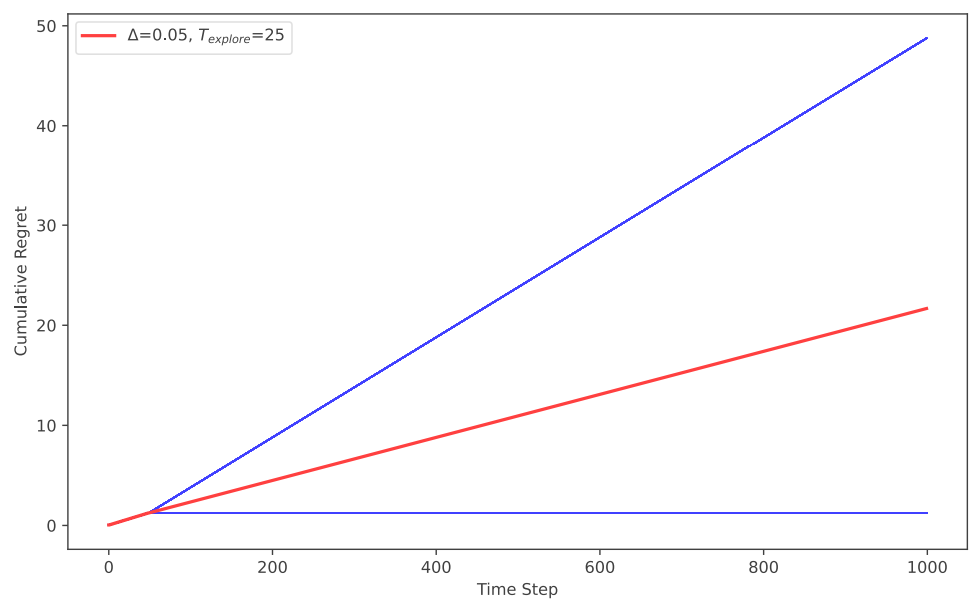
\includegraphics[width=0.33\linewidth]{images/img_20260930_191449.png}
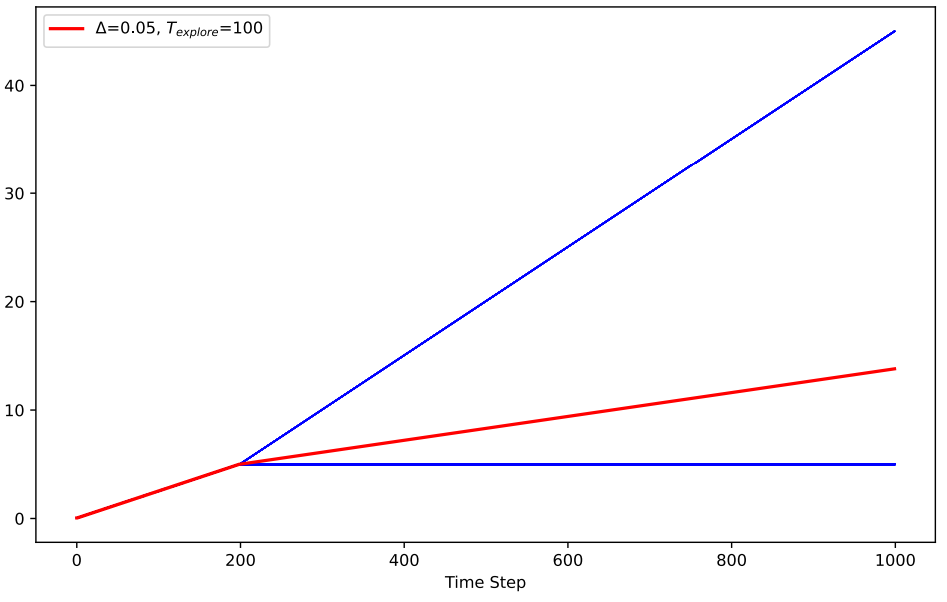
\includegraphics[width=0.32\linewidth]{images/img_20260930_191514.png}
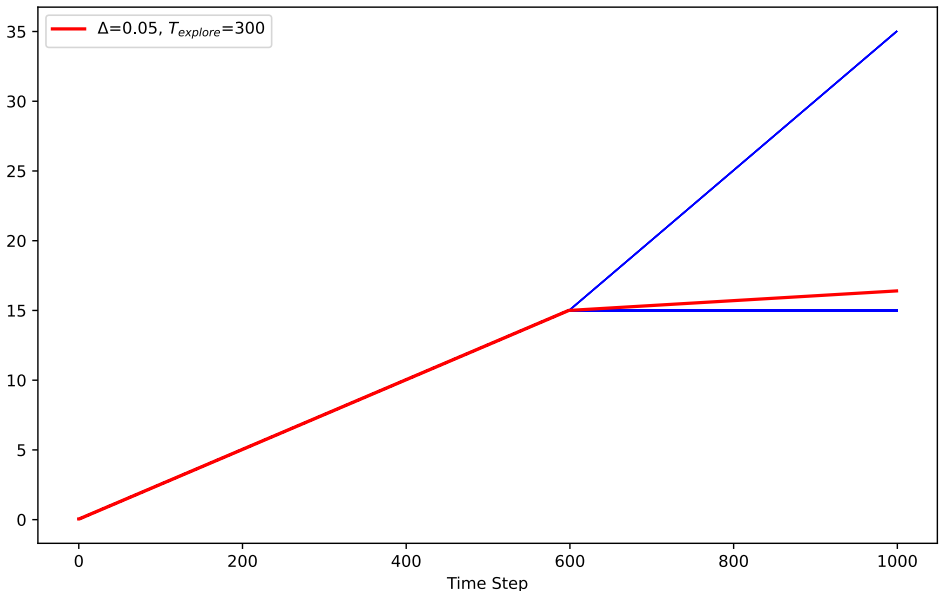
\includegraphics[width=0.32\linewidth]{images/img_20260930_191523.png}
\end{center}

\subsubsection*{Confidence intervals of the per-arm reward}

Recall the confidence interval $\left[\hat{\mu} - \sqrt{\tfrac{2\sigma^2\ln(2/\delta)}{m}},\; \hat{\mu} + \sqrt{\tfrac{2\sigma^2\ln(2/\delta)}{m}}\right]$ after $m$ pulls. As $m$ grows ($m = 25$, $100$, $300$), the intervals around $\mu_1$ and $\mu_2$ shrink until they no longer overlap: the algorithm can then tell the arms apart reliably.

\begin{center}
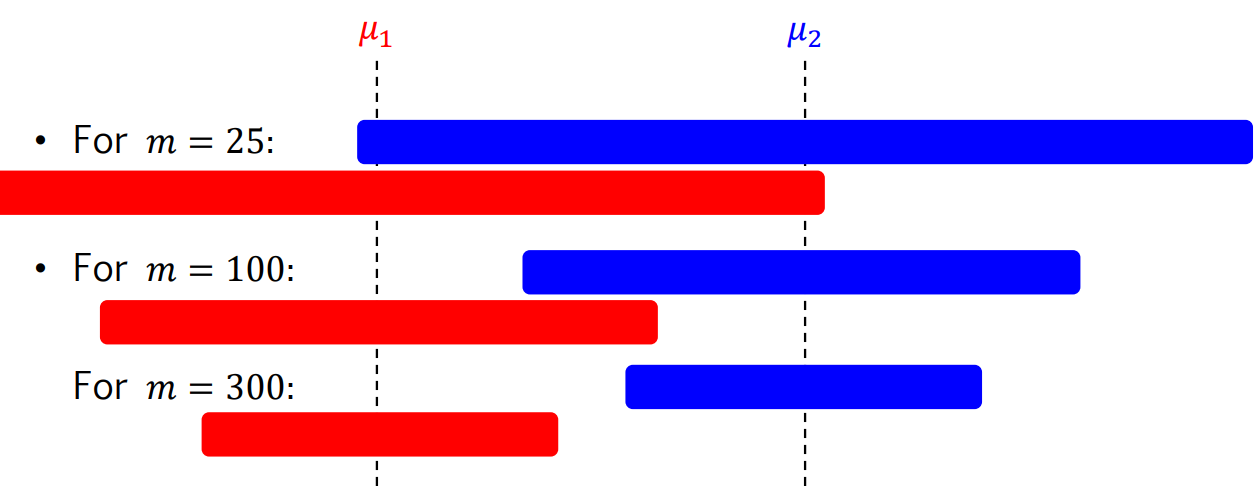
\includegraphics[width=0.7\linewidth]{images/img_20260930_193517.png}
\end{center}

\subsubsection*{Large gap $\Delta = 0.25$}

\begin{itemize}
    \item \textbf{Small $m = 25$}: a larger $\Delta$ means the winning arm is more likely to be the better arm, even with few samples.
    \item \textbf{Large $m = 300$}: no more failures in the simulation.
\end{itemize}

\begin{center}
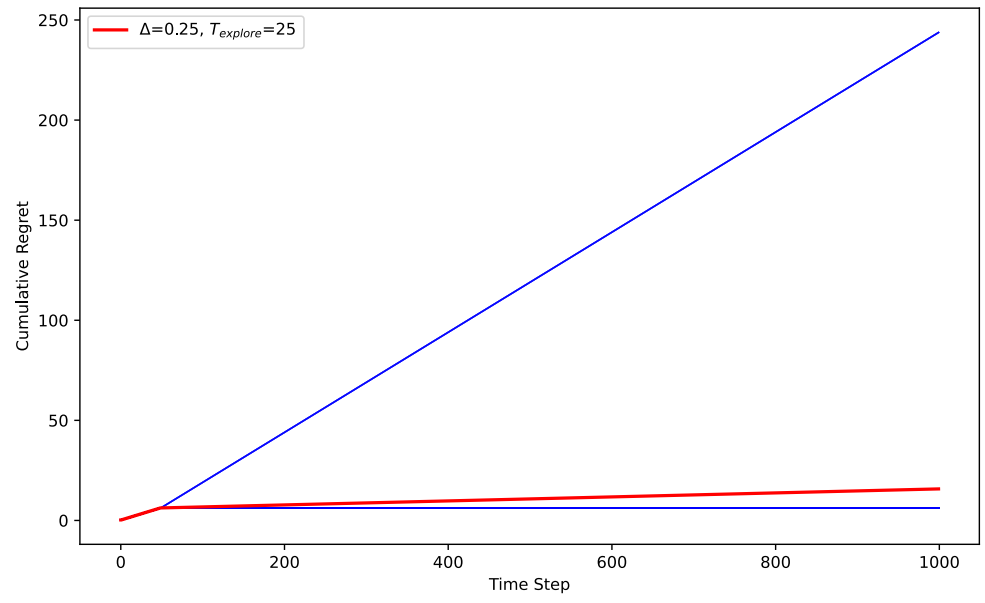
\includegraphics[width=0.48\linewidth]{images/img_20260930_193915.png}
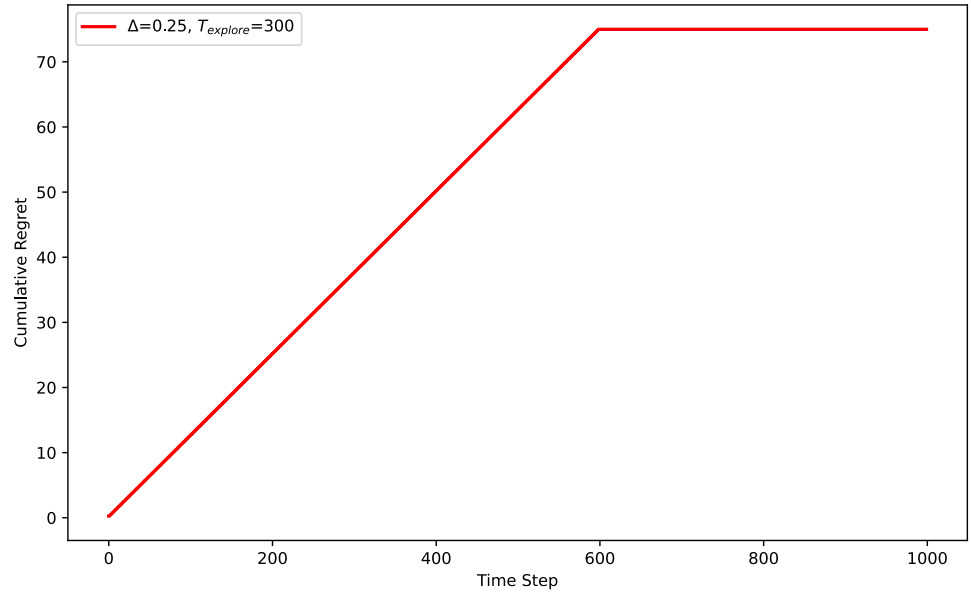
\includegraphics[width=0.48\linewidth]{images/img_20260930_193943.png}
\end{center}

\subsubsection*{Effect of $\Delta$ and $m$}

\begin{itemize}
    \item \textbf{Cumulative regret $R_n$ for different $\Delta$ (fixed $m = 100$)}: a larger $\Delta$ means more costly exploration (each pull of the bad arm costs $\Delta$), but less risky exploitation (the wrong arm is rarely selected).
    \item \textbf{$\mathbb{P}(\text{wrong arm at time } n)$ as a function of $\Delta$ and $m$}: increasing $m$ helps finding the optimal arm; this is made harder by a smaller $\Delta$.
    \item \textbf{Cumulative regret $R_n$ as a function of $\Delta$ and $m$}: there is a tradeoff. For small $\Delta$ one needs a large $m$; for large $\Delta$ a small $m$ suffices. Intermediate $\Delta$ gives a higher regret than both the small and the large $\Delta$ regimes.
\end{itemize}

\begin{center}
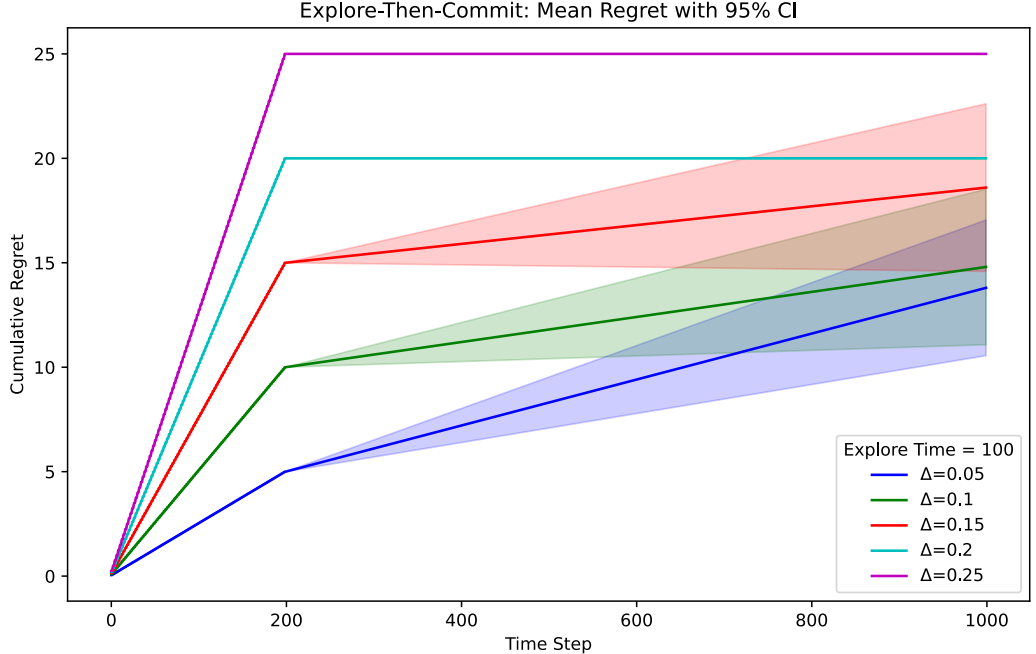
\includegraphics[width=0.7\linewidth]{images/img_20260930_194340.png}
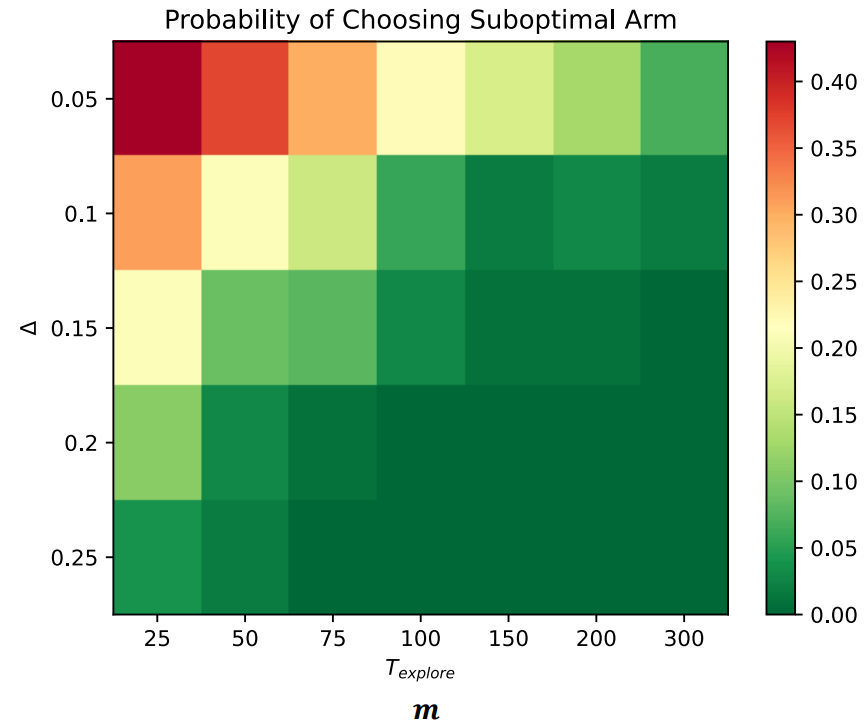
\includegraphics[width=0.45\linewidth]{images/img_20260930_194411.png}
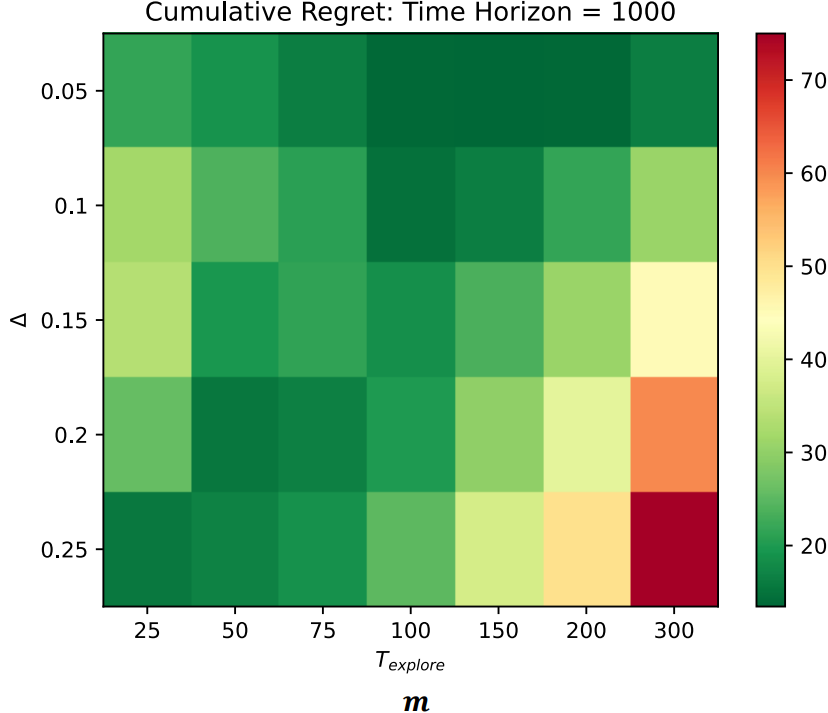
\includegraphics[width=0.45\linewidth]{images/img_20260930_194427.png}
\end{center}

\subsection{Regret bound for ETC with $1$-subgaussian rewards}

\begin{theorem}[Regret of ETC]
For ETC on a $1$-subgaussian bandit (all arms have $1$-subgaussian reward noise), for $n \geq mk$,
\[
R_n \leq \underbrace{m\sum_{i=1}^k \Delta_i}_{\text{exploration}} + \underbrace{(n - mk)\sum_{i=1}^k \Delta_i \exp\left(-\frac{m\Delta_i^2}{4}\right)}_{\text{exploitation}}.
\]
\end{theorem}

\begin{proof}
Assume without loss of generality that $\mu_1 = \mu^* = \max_i \mu_i$ (so $\Delta_1 = 0$). By the regret decomposition lemma (previous lecture),
\[
R_n = \sum_{i=1}^k \Delta_i\, \mathbb{E}[T_i(n)].
\]
Arm $i$ is pulled exactly $m$ times during exploration; afterwards, it is pulled at each of the $n - mk$ remaining steps if and only if it was selected at time $mk+1$. Hence
\begin{align*}
\mathbb{E}[T_i(n)] &= m + (n - mk)\,\mathbb{P}\big(A_{mk+1} = i\big) \\
&\leq m + (n - mk)\,\mathbb{P}\Big(\hat{\mu}_i(mk) \geq \max_{j \neq i}\hat{\mu}_j(mk)\Big).
\end{align*}
Now, for $i \neq 1$, the event that $i$ beats \emph{all} other arms is contained in the event that it beats arm $1$:
\begin{align*}
\mathbb{P}\Big(\hat{\mu}_i(mk) \geq \max_{j \neq i}\hat{\mu}_j(mk)\Big) &\leq \mathbb{P}\big(\hat{\mu}_i(mk) \geq \hat{\mu}_1(mk)\big) \\
&= \mathbb{P}\Big(\big(\hat{\mu}_i(mk) - \mu_i\big) - \big(\hat{\mu}_1(mk) - \mu_1\big) \geq \Delta_i\Big).
\end{align*}
The empirical mean $\hat{\mu}_i(mk)$ is computed from $m$ i.i.d.\ samples: $m\hat{\mu}_i - m\mu_i$ is a sum of $m$ independent $1$-subgaussian variables, hence $m\hat{\mu}_i(mk)$ is $\sqrt{m}$-subgaussian, so $\hat{\mu}_i(mk) - \mu_i$ is $1/\sqrt{m}$-subgaussian. The two arms are sampled independently, so the difference $\big(\hat{\mu}_i - \mu_i\big) - \big(\hat{\mu}_1 - \mu_1\big)$ is $\sqrt{2/m}$-subgaussian. The tail bound then gives
\[
\mathbb{P}\Big(\big(\hat{\mu}_i - \mu_i\big) - \big(\hat{\mu}_1 - \mu_1\big) \geq \Delta_i\Big) \leq \exp\left(-\frac{\Delta_i^2}{2\cdot(2/m)}\right) = \exp\left(-\frac{m\Delta_i^2}{4}\right).
\]
Plugging everything back into $R_n = \sum_i \Delta_i\,\mathbb{E}[T_i(n)]$ gives the claim.
\end{proof}

\begin{remark}[Tradeoff]

\begin{itemize}
    \item $m$ large $\Rightarrow$ exploration is costly (first term grows linearly in $m$);
    \item $m$ small $\Rightarrow$ potential to bet on the wrong arm forever (second term is large, it is multiplied by $n - mk$).
\end{itemize}
This is exactly the explore-exploit tradeoff, now quantified.
\end{remark}

\subsection{Analysis for $k = 2$}

Assume again that the first arm is optimal: $\Delta_1 = 0$, and write $\Delta_2 = \Delta$. The bound for general $k$ becomes
\[
R_n \leq m\Delta + (n - 2m)\Delta\exp\left(-\frac{m\Delta^2}{4}\right) \leq m\Delta + n\Delta\exp\left(-\frac{m\Delta^2}{4}\right).
\]

\textbf{Which $m$ minimizes this quantity?} Differentiating the right-hand side with respect to $m$:
\[
\Delta - n\Delta\cdot\frac{\Delta^2}{4}\exp\left(-\frac{m\Delta^2}{4}\right) = 0 \iff \exp\left(-\frac{m\Delta^2}{4}\right) = \frac{4}{n\Delta^2},
\]
so (ignoring rounding)
\[
m = \frac{4}{\Delta^2}\ln\left(\frac{n\Delta^2}{4}\right).
\]
The resulting regret bound is of the form
\[
R_n \leq \Delta + C\sqrt{n},
\]
for a universal constant $C$.

\begin{itemize}
    \item Without an assumption on $\Delta$, we cannot avoid potentially infinite regret (a single bad pull can cost arbitrarily much). Within a bandit class such that $\Delta \leq 1$: $R_n \leq 1 + C\sqrt{n}$.
    \item Replacing $\Delta$ by a value result in an example of a \textbf{worst-case} (or \textbf{problem-independent}) bound: it does not depend on the specific environment instance $\nu$, only on the environment class (here: subgaussian and $\Delta \leq 1$) and on the horizon $n$.
    \item \textbf{But}: to set the correct $m$, we do need to know $\Delta$ ``ahead of time''. Can we have a universal algorithm that does well for unknown $\Delta$, i.e., that decides \emph{adaptively} when we have explored enough? (This motivates the algorithms of the next lectures.)
\end{itemize}

\subsection{Comparison of the bound with simulations}

The bound is relatively loose (due to approximations in the proof) for intermediate suboptimality gaps $\Delta$, but pretty good for larger $\Delta$. It slightly underestimates the critical $\Delta$ (the gap at which the actual regret peaks).

\begin{center}
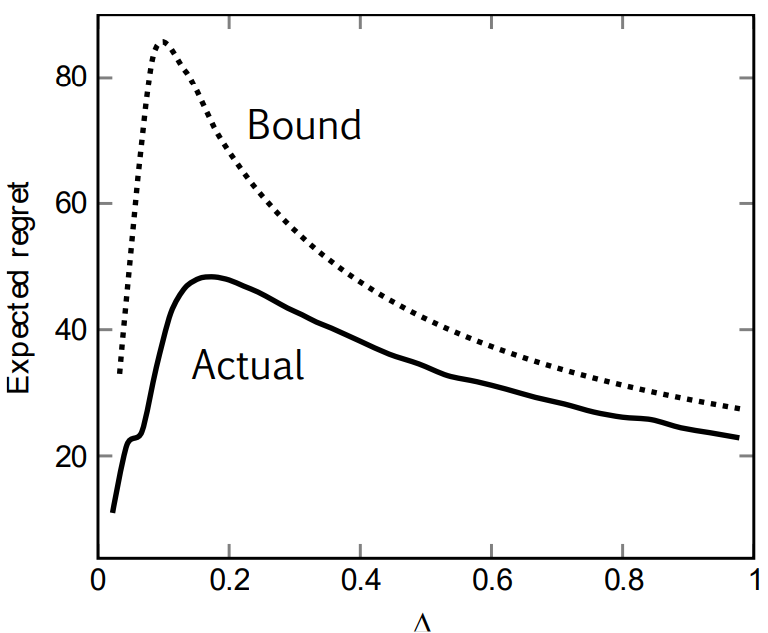
\includegraphics[width=0.5\linewidth]{images/img_20260930_202641.png}
\end{center}

\section{Summary}

\begin{itemize}
    \item \textbf{Convergence of random variables}: for sums of i.i.d.\ variables, the law of large numbers and the central limit theorem describe the asymptotic behavior. Markov and Chebyshev give finite-$n$ bounds, but they are too loose ($1/n$).
    \item \textbf{Tail bound for finite $n$}: the large deviation (Chernoff-type) bound $\mathbb{P}(\hat{\mu} \geq \mu + \epsilon) \leq \exp(-n\epsilon^2/(2\sigma^2))$, valid for subgaussian noise, and the resulting confidence intervals of width $\sqrt{2\sigma^2\ln(2/\delta)/n}$.
    \item \textbf{Subgaussian distributions}: ``nice'' noise, light tail, ``no big excesses''. It is a strong condition (even the exponential distribution is too heavy). Properties: scaling ($\alpha X$ is $|\alpha|\sigma$-subgaussian) and independent sums (variance parameters add up). Examples: Gaussian, bounded variables.
    \item \textbf{Explore-then-Commit (ETC)}: explore for a fixed window ($m$ pulls per arm), then exploit forever. Tradeoff between expensive exploration and failed exploitation.
    \item \textbf{Upper bound on $R_n$ for the $1$-subgaussian bandit}: $R_n \leq m\sum_i\Delta_i + (n - mk)\sum_i\Delta_i\exp(-m\Delta_i^2/4)$; for $k = 2$ and optimally tuned $m$, $R_n \leq \Delta + C\sqrt{n}$. Limitation: tuning $m$ requires knowing $\Delta$.
\end{itemize}
